\begin{name}
{Biên soạn: Dương Phước Sang \\ Phản biện: Dương Công Tạo}
{Đề ôn tập chương I}
\end{name}

\caulc
\Opensolutionfile{ans}[ans/ans\currfilebase-Phan-I]
\begin{ex}%[2-D1B5-SO-16-2425]%[VN-MT-7, Dương Phước Sang]%[2D1H1-1]
Hàm số $y=x^3-3x^2+2$ đồng biến trên khoảng nào dưới đây?
\choice
{\True $(-2;0)$}
{$(0;+\infty)$}
{$(-\infty;2)$}
{$(0;2)$}
\loigiai{
Ta có $y'=3x^2-6x$.\\
$y' \geq 0 \Leftrightarrow 3x^2-6x \geq 0 \Leftrightarrow \hoac{&x \geq 2\\&x \leq 0.}$\\
Suy ra hàm số đồng biến trên các khoảng $(-\infty;0)$ và $(2;+\infty)$ nên đồng biến trên khoảng $(-2;0)$.
}
\end{ex}

\begin{ex}%[2-D1B5-SO-16-2425]%[VN-MT-7, Dương Phước Sang]%[2D1H2-1]
Cho hàm số $y=27x^3+108x^2-81x+189$. Điểm cực tiểu của hàm số là
\choice
{$-3$}
{\True $\dfrac{1}{3}$}
{$175$}
{$675$}
\loigiai{
Ta có $y'=81x^2+216x-81$.\\
$y'=0 \Leftrightarrow \hoac{&x=\dfrac{1}{3}\\&x=-3.}$
\begin{center}

\begin{tikzpicture}
\tkzTabInit[nocadre=true,lgt=1.2,espcl=2.5,deltacl=0.6]
{$x$/0.7, $y'$/0.6, $y$/2}
{$-\infty$,$-3$,$\tfrac{1}{3}$,$+\infty$}
\tkzTabLine{,+,0,-,0,+,}
\tkzTabVar{-/,+/,-/,+/}
\end{tikzpicture}
\end{center}
Vậy điểm cực tiểu của hàm số là $x_{_\text{CT}}=\dfrac{1}{3}$.
}
\end{ex}

\begin{ex}%[2-D1B5-SO-16-2425]%[VN-MT-7, Dương Phước Sang]%[2D1H3-1]
Giá trị lớn nhất của hàm số $f(x)=x^3-8x^2+16x-9$ trên đoạn $[1;3]$ là
\choice
{$\max\limits_{[1; 3]} f(x)=0$}
{\True $\max\limits_{[1; 3]} f(x)=\dfrac{13}{27}$}
{$\max\limits_{[1; 3]} f(x)=-6$}
{$\max\limits_{[1; 3]} f(x)=5$}
\loigiai{
Hàm số $f(x)$ liên tục trên $[1;3]$.\\
Ta có $f'(x)=3x^2-16x+16$; $f'(x)=0 \Leftrightarrow \hoac{&x=4 \notin (1;3)\\&x=\dfrac{4}{3}\in (1;3).}$\\
$f(1)=0$; $f\left( \dfrac{4}{3} \right)=\dfrac{13}{27}$; $f(3)=-6$.\\
Do đó $\max\limits_{x \in [1;3]} f(x)=f\left( \dfrac{4}{3} \right)=\dfrac{13}{27}$.
}
\end{ex}

\begin{ex}%[2-D1B5-SO-16-2425]%[VN-MT-7, Dương Phước Sang]%[2D1H3-1]
Giá trị lớn nhất của hàm số $f(x)=x^4-4x^2+1$ trên đoạn $[1;3]$ bằng
\choice
{\True $46$}
{$64$}
{$3$}
{$\sqrt{2}$}
\loigiai{
Ta có hàm số $f(x)=x^4-4x^2+1$ liên tục trên đoạn $[1;3]$.\\
$f'(x)=4x^3-8x$.\\
$f'(x)=0 \Leftrightarrow 4x^3-8x=0 \Leftrightarrow \hoac{&x=0 \notin (1;3)\\&x=\sqrt{2} \in (1;3)\\&x=-\sqrt{2} \notin (1;3).}$\\
$f(1)=-2$; $f\left( \sqrt{2} \right)=-3$; $f(3)=46$.\\
Vậy giá trị lớn nhất của hàm đã cho trên đoạn $[1;3]$ bằng $46$.
}
\end{ex}

\begin{ex}%[2-D1B5-SO-16-2425]%[VN-MT-7, Dương Phước Sang]%[2D1N4-1]
Tiệm cận ngang của đồ thị hàm số $y=\dfrac{2x+3}{x-1}$ là
\choice
{$y=1$}
{\True $y=2$}
{$x=1$}
{$x=2$}
\loigiai{
Tập xác định của hàm số là $\mathscr{D}=\mathbb{R} \setminus \{1\}$.\\
Ta có 
$\lim\limits_{x \to \pm\infty} y=\lim\limits_{x \to \pm\infty} \dfrac{2x+3}{x-1}=\lim\limits_{x \to \pm\infty} \dfrac{2+\dfrac{3}{x}}{1-\dfrac{1}{x}}=2$.\\
Vậy đồ thị của hàm số có tiệm cận ngang là đường thẳng $y=2$.
}
\end{ex}

\begin{ex}%[2-D1B5-SO-16-2425]%[VN-MT-7, Dương Phước Sang]%[2D1N4-1]
Tiệm cận đứng của đồ thị hàm số $y=\dfrac{2x+1}{x-1}$ là
\choice
{\True $x=1$}
{$y=2$}
{$x=2$}
{$x=-1$}
\loigiai{
Tập xác định của hàm số $\mathscr{D}=\mathbb{R} \setminus \{1\}$.\\
Ta có 
$\lim\limits_{x \to 1^+} y=\lim\limits_{x \to 1^+} \dfrac{2x+1}{x-1}=\lim\limits_{x \to 1^+} \left(2+\dfrac{3}{x-1}\right)=+\infty$.\\
Vậy đồ thị của hàm số có tiệm cận đứng là đường thẳng $x=1$.
}
\end{ex}

\begin{ex}%[2-D1B5-SO-16-2425]%[VN-MT-7, Dương Phước Sang]%[2D1H4-1]
Đường thẳng nào sau đây là tiệm cận xiên của đồ thị hàm số $y=\dfrac{2x^2-3x+1}{x+2}$?
\choice
{$y=2x$}
{$y=2$}
{\True $y=2x-7$}
{$x=-2$}
\loigiai{
Ta có $y=f(x)=\dfrac{2x^2-3x+1}{x+2}=2x-7+\dfrac{15}{x+2}$.\\
$\lim\limits_{x \to \pm\infty} [f(x)-(2x-7)]=\lim\limits_{x \to \pm\infty} \dfrac{15}{x+2}=0$.\\
Vậy đồ thị hàm số có tiệm cận xiên là $y=2x-7$.
}
\end{ex}

\begin{ex}%[2-D1B5-SO-16-2425]%[VN-MT-7, Dương Phước Sang]%[2D1N1-2]
Cho hàm số $y=f(x)$ có bảng biến thiên như sau:
\begin{center}

\begin{tikzpicture}
\tkzTabInit[nocadre=true,lgt=1.2,espcl=2.5,deltacl=0.6]
{$x$/0.6, $y'$/0.6, $y$/2}
{$-\infty$,$-2$,$0$,$+\infty$}
\tkzTabLine{,+,0,-,0,+,}
\tkzTabVar{-/$-\infty$,+/$1$,-/$-3$,+/$+\infty$}
\end{tikzpicture} 
\end{center}
Hàm số $y=f(x)$ nghịch biến trên khoảng nào dưới đây?
\choice
{$(-\infty;-2)$}
{$(0;+\infty)$}
{$(-3;1)$}
{\True $(-2;0)$}
\loigiai{
Dựa vào bảng biến thiên, ta thấy $f'(x)<0 \Leftrightarrow x \in (-2;0)$ nên hàm số nghịch biến trên khoảng $(-2;0)$.
}
\end{ex}

\begin{ex}%[2-D1B5-SO-16-2425]%[VN-MT-7, Dương Phước Sang]%[2D1H5-1]
Cho bảng biến thiên của hàm số $y=f(x)$ như sau:
\begin{center}

\begin{tikzpicture}
\tikzset{double style/.append style={double distance=1.5pt}}
\tkzTabInit[nocadre=true,lgt=1.2,espcl=4,deltacl=0.6]
{$x$/0.6,$y'$/0.6,$y$/2}
{$-\infty$,$1$,$+\infty$}
\tkzTabLine{,-,d,-,}
\tkzTabVar{+/$1$,-D+/$-\infty$/$+\infty$,-/$1$}
\end{tikzpicture} 
\end{center}
Hỏi đây là bảng biến thiên của hàm số nào trong các hàm số sau?
\choice
{$y=\dfrac{x-3}{x-1}$}
{$y=\dfrac{-x+2}{x-1}$}
{$y=\dfrac{x+2}{x+1}$}
{\True $y=\dfrac{x+2}{x-1}$}
\loigiai{
Bảng biến thiên được cung cấp có đặc điểm:
\begin{itemize}
\item Đồ thị hàm số có đường tiệm cận đứng là $x=1$, loại $y=\dfrac{x+2}{x+1}$.
\item Đồ thị hàm số có đường tiệm cận ngang là $y=1$, loại $y=\dfrac{-x+2}{x-1}$.
\item $y'<0,\,\forall x \ne 1$, trong khi $\left(\dfrac{x-3}{x-1}\right)'=\dfrac{2}{(x-1)^2}>0,\,\forall x \neq 1$, loại $y=\dfrac{x-3}{x-1}$.
\end{itemize}
Chỉ có hàm số $y=\dfrac{x+2}{x-1}$ thỏa mãn các đặc điểm trên.
}
\end{ex}

\begin{ex}%[2-D1B5-SO-16-2425]%[VN-MT-7, Dương Phước Sang]%[2D1H1-1]
Cho hàm số $y=\dfrac{x^2-2x}{1-x}$. Khẳng định nào sau đây đúng?
\choice
{Hàm số đồng biến trên $\mathbb{R}$}
{\True Hàm số nghịch biến trên các khoảng $(-\infty;1)$ và $(1;+\infty)$}
{Hàm số nghịch biến trên $\mathbb{R}$}
{Hàm số đồng biến trên các khoảng $(-\infty;1)$ và $(1;+\infty)$}
\loigiai{
Tập xác định $\mathscr{D}=\mathbb{R} \setminus \big\{1\big\}$.\\
$y'=\dfrac{-x^2+2x-2}{(1-x)^2}=\dfrac{-(x-1)^2-1}{(1-x)^2}<0,\,\forall x \in \mathscr{D}$.\\
Vậy hàm số nghịch biến trên các khoảng $(-\infty;1)$ và $(1;+\infty)$.
}
\end{ex}

\begin{ex}%[2-D1B5-SO-16-2425]%[VN-MT-7, Dương Phước Sang]%[1D7H2-8]
Cho chuyển động được xác định bởi phương trình $s(t)=3t^3+4t^2-t$, trong đó $t$ được tính bằng giây (s) và $s(t)$ được tính bằng mét. Vận tốc của chuyển động khi $t=4$\,s bằng
\choice
{\True $175$ m/s}
{$41$ m/s}
{$176$ m/s}
{$20$ m/s}
\loigiai{
Ta có $v(t)=s'(t)=9t^2+8t-1$.\\
Vận tốc của chuyển động khi $t=4$\,s bằng $v(4)=9 \cdot 4^2+8 \cdot 4-1=175$ m/s.
}
\end{ex}

\begin{ex}%[2-D1B5-SO-16-2425]%[VN-MT-7, Dương Phước Sang]%[2D1H2-1]
Cho hàm số $y=f(x)$ có đạo hàm $f'(x)=x^2(x-1)$ với mọi số thực $x$. Số điểm cực tiểu của hàm số $f(x)$ là
\choice
{$0$}
{\True $1$}
{$2$}
{$3$}
\loigiai{
Ta có $f'(x)=x^2(x-1)=0 \Leftrightarrow \hoac{&x=0&&\text{(nghiệm kép)}\\&x=1.}$\\
Bảng biến thiên:
\begin{center}

\begin{tikzpicture}
\tkzTabInit[nocadre=true,lgt=1.2,espcl=2.5,deltacl=0.6]
{$x$/0.6, $f'(x)$/0.6, $f(x)$/2}
{$-\infty$,$0$,$1$,$+\infty$}
\tkzTabLine{,-,0,-,0,+,}
\tkzTabVar{+/,R,-/,+/}
\end{tikzpicture} 
\end{center}
Từ bảng biến thiên ta thấy hàm số có một điểm cực tiểu duy nhất là $x=1$.
}
\end{ex}
\Closesolutionfile{ans}

\cauds
\Opensolutionfile{ans}[ans/ans\currfilebase-Phan-II]
\begin{ex}%[2-D1B5-SO-16-2425]%[VN-MT-7, Dương Phước Sang]%[2D1V2-1]
Cho các hàm số $f(x)=x^3-3x^2+2025$ và $g(x)=\dfrac{x^2-2x+1}{x-2}$.
\choiceTF
{\True Hàm số $y=f(x)$ nghịch biến trên khoảng $(0;2)$}
{Hàm số $y=g(x)$ nghịch biến trên khoảng $(1;3)$}
{\True Điểm cực đại của hàm số $y=f(x)$ là $x=0$}
{\True Đường thẳng đi qua $2$ điểm cực trị của đồ thị hàm số $y=g(x)$ cũng đi qua điểm $N(2;2)$}
\loigiai{
\begin{itemchoice}
\itemch \textbf{Đúng}.\\
Với $f(x)=x^3-3x^2+2025$, ta có $f'(x)=3x^2-6x$ và $f'(x)=0 \Leftrightarrow \hoac{&x=0\\&x=2.}$\\
Từ đó, ta có bảng xét dấu của $f'(x)$ như sau:
\begin{center}

\begin{tikzpicture}
\tkzTabInit[nocadre=true,lgt=1.2,espcl=2,deltacl=0.6]
{$x$/0.6,$f'(x)$/0.6}
{$-\infty$,$0$,$2$,$+\infty$}
\tkzTabLine{,+,0,-,0,+,}
\end{tikzpicture}
\end{center}
Suy ra hàm số nghịch biến trên khoảng $(0;2)$.
\itemch \textbf{Sai}.\\
Hàm số $y=g(x)=\dfrac{x^2-2x+1}{x-2}$ có tập xác định: $\mathscr{D}=\mathbb{R} \setminus \big\{2\big\}$.\\
Ta có $y'=\dfrac{x^2-4x+3}{(x-2)^2}$ và $y'=0 \Leftrightarrow x^2-4x+3=0 \Leftrightarrow \hoac{&x=1\\&x=3.}$\\
Bảng xét dấu của $g'(x)$:
\begin{center}

\begin{tikzpicture}
\tikzset{double style/.append style={double distance=1.5pt}}
\tkzTabInit[nocadre=true,lgt=1.2,espcl=2.5,deltacl=0.6]
{$x$/0.6,$g'(x)$/0.6}
{$-\infty$,$1$,$2$,$3$,$+\infty$}
\tkzTabLine{,+,0,-,d,-,0,+,}
\end{tikzpicture}
\end{center}
Suy ra hàm số nghịch biến trên khoảng $(1;2)$ và $(2;3)$.
\itemch \textbf{Đúng}.\\
Với $f(x)=x^3-3x^2+2025$, ta có $f'(x)=3x^2-6x$ và $f'(x)=0 \Leftrightarrow \hoac{&x=0\\&x=2.}$\\
Bảng biến thiên của hàm số $y=f(x)$:
\begin{center}

\begin{tikzpicture}
\tkzTabInit[nocadre=true,lgt=1.2,espcl=2.5,deltacl=0.6]
{$x$/0.6, $f'(x)$/0.6, $f(x)$/2}
{$-\infty$,$0$,$2$,$+\infty$}
\tkzTabLine{,+,0,-,0,+,}
\tkzTabVar{-/,+/,-/,+/}
\end{tikzpicture}
\end{center}
Suy ra điểm cực đại của hàm số là $x=0$.
\itemch \textbf{Đúng}.\\
Hàm số $y=g(x)=\dfrac{x^2-2x+1}{x-2}$ có tập xác định: $\mathscr{D}=\mathbb{R} \setminus \big\{2\big\}$.\\
Ta có $y'=\dfrac{x^2-4x+3}{(x-2)^2}$ và $y'=0 \Leftrightarrow x^2-4x+3=0 \Leftrightarrow \hoac{&x=1\\&x=3.}$\\
Bảng biến thiên của $g(x)$:
\begin{center}

\begin{tikzpicture}
\tikzset{double style/.append style={double distance=1.5pt}}
\tkzTabInit[nocadre=true,lgt=1.2,espcl=2.5,deltacl=0.6]
{$x$/0.6,$y'$/0.6,$y$/2}
{$-\infty$,$1$,$2$,$3$,$+\infty$}
\tkzTabLine{,+,0,-,d,-,0,+,}
\tkzTabVar{-/$-\infty$,+/$0$,-D+/$-\infty$/$+\infty$,-/$4$,+/$+\infty$}
\end{tikzpicture}
\end{center}
Hai điểm cực trị của đồ thị hàm số $y=g(x)$ là $A(1;0)$ và $B(3;4)$, cùng thuộc $AB\colon y=2x-2$.\\
Đường thẳng $AB$ đó đi qua điểm $N(2;2)$.
\end{itemchoice}
}
\end{ex}

\begin{ex}%[2-D1B5-SO-16-2425]%[VN-MT-7, Dương Phước Sang]%[2D1V3-1]
Cho các hàm số $f(x)=x^3-8x^2+16x-9$ và $h(x)=\dfrac{x^2-x+1}{x-1}$.
\choiceTF
{\True Giá trị lớn nhất của hàm số $y=f(x)$ trên đoạn $[-1;1]$ là $0$}
{Gọi giá trị lớn nhất và giá trị nhỏ nhất của hàm số $y=f(x)$ trên đoạn $[1;3]$ lần lượt là $a$, $b$. Khi đó giá trị của $27a-b$ bằng $13$}
{\True Giá trị nhỏ nhất của hàm số $y=h(x)$ trên khoảng $(1;+\infty)$ là $3$}
{\True Giá trị nhỏ nhất của hàm số $y=f\big(h(x)\big)$ trên khoảng $(1;3)$ là $-9$}
\loigiai{
\begin{itemchoice}
\itemch \textbf{Đúng}.\\
Với $f(x)=x^3-8x^2+16x-9$, ta có $f'(x)=3x^2-16x+16$.\\
Cho $f'(x)=0 \Leftrightarrow 3x^2-16x+16=0 \Leftrightarrow \hoac{&x=4 \notin [-1;1]\\&x=\dfrac{4}{3} \notin [-1;1].}$\\
Do $\heva{&f(-1)=-34\\&f(1)=0}$ nên $\max\limits_{x \in [-1;1]} f(x) =0$.
\itemch \textbf{Sai}.\\
Với $f(x)=x^3-8x^2+16x-9$, ta có $f'(x)=3x^2-16x+16$.\\
Cho $f'(x)=0 \Leftrightarrow 3x^2-16x+16=0 \Leftrightarrow \hoac{&x=4 \notin [1;3]\\&x=\dfrac{4}{3} \in [1;3].}$\\
Vì $\heva{&f(1)=0\\&f(\dfrac{4}{3})=\dfrac{13}{27}\\&f(3)=-6}$ nên $\heva{&\max\limits_{x \in [1;3]} f(x) =\dfrac{13}{27}=a\\&\min\limits_{x \in [1;3]} f(x) =-6=b}$. Từ đó $27a-b=19$.
\itemch \textbf{Đúng}.\\
Với $h(x)=\dfrac{x^2-x+1}{x-1}$, ta có $h'(x)=\dfrac{x^2-2x}{(x-1)^2}$.\\
Cho $h'(x)=0 \Rightarrow x^2-2x=0 \Leftrightarrow \hoac{&x=0 \notin (1;+\infty)\\&x=2 \in (1;+\infty).}$
\begin{center}

\begin{tikzpicture}
\tkzTabInit[nocadre=true,lgt=1.2,espcl=2.5,deltacl=0.6]
{$x$/0.6,$h'(x)$/0.6,$h(x)$/2}
{$1$,$2$,$+\infty$}
\tkzTabLine{,-,0,+,}
\tkzTabVar{+/$+\infty$,-/$3$,+/$+\infty$}
\end{tikzpicture}
\end{center}
Từ bảng biến thiên, suy ra giá trị nhỏ nhất của hàm số $y=h(x)$ trên khoảng $(1;+\infty)$ là $3$.
\itemch \textbf{Đúng}.\\
Với $t=h(x)=\dfrac{x^2-x+1}{x-1}$, ta có $h'(x)=\dfrac{x^2-2x}{(x-1)^2}$.\\
Cho $h'(x)=0 \Rightarrow x^2-2x=0 \Leftrightarrow \hoac{&x=0 \notin (1;3)\\&x=2 \in (1;3).}$
\begin{center}
 
\begin{tikzpicture}
 \tkzTabInit[nocadre=true,lgt=1.2,espcl=2.5,deltacl=0.6]
 {$x$/0.6,$h'(x)$/0.6,$h(x)$/2}
 {$1$,$2$,$3$}
 \tkzTabLine{,-,0,+,}
 \tkzTabVar{+/$+\infty$,-/$3$,+/$\tfrac{7}{2}$}
 \end{tikzpicture}
\end{center}
Như thế đặt $t=h(x)$, $x\in (1;3)$ thì $t \in [3;+\infty)$ và $y=f(t)=t^3-8t^2+16t-9$.\\
Ta có $f'(t)=3t^2-16t+16$.\\
Cho $f'(t)=0 \Leftrightarrow 3t^2-16t+16=0 \Leftrightarrow \hoac{&t=4 \in [3;+\infty)\\&x=\dfrac{4}{3} \notin [3;+\infty).}$
\begin{center}
 
\begin{tikzpicture}
 \tkzTabInit[nocadre=true,lgt=1.2,espcl=2.5,deltacl=0.6]
 {$t$/0.6,$f'(t)$/0.6,$f(t)$/2}
 {$3$,$4$,$+\infty$}
 \tkzTabLine{,-,0,+,}
 \tkzTabVar{+/$-6$,-/$-9$,+/$+\infty$}
 \end{tikzpicture}
\end{center}
Vậy $\min\limits_{1<x<3} f\big(h(x)\big)=\min\limits_{t \geq 3} f(t)=f(4)=-9$.
\end{itemchoice}
}
\end{ex}

\begin{ex}%[2-D1B5-SO-16-2425]%[VN-MT-7, Dương Phước Sang]%[2D1V4-1]
Cho các hàm số $f(x)=\dfrac{x-2}{x+3}$ và $g(x)=\dfrac{x^2-3x}{x+1}$. 
\choiceTF
{\True Đồ thị hàm số $y=f(x)$ có đường tiệm cận ngang là đường thẳng $y=1$}
{\True Đồ thị hàm số $y=g(x)$ có đường tiệm cận đứng là đường thẳng $x=-1$}
{\True Đồ thị hàm số $y=g(x)$ có đường tiệm cận xiên là đường thẳng $y=x-4$}
{\True Đồ thị hàm số $y=g\big(f(x)\big)$ không có đường tiệm cận xiên nào cả}
\loigiai{
\begin{itemchoice}
\itemch \textbf{Đúng}.\\
Ta có $\lim\limits_{x \to \pm\infty} \dfrac{x-2}{x+3}=\lim\limits_{x \to \pm\infty} \dfrac{1-\dfrac{2}{x}}{1+\dfrac{3}{x}}=1$ nên đồ thị hàm số $y=\dfrac{x-2}{x+3}$ có đường tiệm cận ngang là đường thẳng $y=1$.
\itemch \textbf{Đúng}.\\
Ta có $\lim\limits_{x \to -1^+} \dfrac{x^2-3x}{x+1}=\lim\limits_{x \to -1^+} \left(x-4+\dfrac{4}{x+1}\right)=+\infty$ nên đồ thị hàm số $y=\dfrac{x^2-3x}{x+1}$ có đường tiệm cận đứng là đường thẳng $x=-1$.
\itemch \textbf{Đúng}.\\
Ta có $y=\dfrac{x^2-3x}{x+1}=x-4+\dfrac{4}{x+1}$ nên $\lim\limits_{x \to \pm\infty} \left(\dfrac{x^2-3x}{x+1}-(x-4)\right)=\lim\limits_{x \to \pm\infty} \dfrac{4}{x+1}=0$.\\
Vậy đường thẳng $y=x-4$ là tiệm cận xiên của đồ thị hàm số $y=\dfrac{x^2-3x}{x+1}$.
\itemch \textbf{Đúng}.\\
Ta có $y=g\big(f(x)\big)=\dfrac{\big(f(x)\big)^2-3\big(f(x)\big)}{f(x)+1}$ nên $\lim\limits_{x \to \pm\infty} g\big(f(x)\big)=\lim\limits_{x \to \pm\infty} \dfrac{\big(f(x)\big)^2-3\big(f(x)\big)}{f(x)+1}$.\\
Mà $\lim\limits_{x \to \pm\infty} f(x)=\lim\limits_{x \to \pm\infty} \dfrac{x-2}{x+3}=\lim\limits_{x \to \pm\infty} \dfrac{1-\dfrac{2}{x}}{1+\dfrac{3}{x}}=1$ nên
$\lim\limits_{x \to \pm\infty} g\big(f(x)\big)=\dfrac{1^2-3\cdot 1}{1+1}=-1$.\\
Vậy $(C)\colon y=g\big(f(x)\big)$ có tiệm cận ngang $y=-1$ mà không có tiệm cận xiên.
\end{itemchoice}
}
\end{ex}

\begin{ex}%[2D1C4-3]
Cho hàm số $y=f(x)$ xác định trên tập $\mathscr{D}=\mathbb{R} \setminus \{2\}$, có bảng biến thiên như sau:
\begin{center}

\begin{tikzpicture}
\tikzset{double style/.append style={double distance=1.5pt}}
\tkzTabInit[nocadre=true,lgt=1.2,espcl=2]
{$x$/0.6,$f'(x)$/0.6,$f(x)$/2}
{$-\infty$,$1$,$2$,$3$,$+\infty$}
\tkzTabLine{,+,0,-,d,-,0,+,}
\tkzTabVar{-/$-\infty$,+/$1$,-D+/$-\infty$/$+\infty$,-/$5$,+/$+\infty$}
\end{tikzpicture}
\end{center}
\choiceTF
{\True Hàm số $y=f(x)$ có cực đại nhỏ hơn cực tiểu}
{\True Hàm số $f(x)=\dfrac{x^2-x-1}{x-2}$ có bảng biến thiên như trên}
{\True Đồ thị hàm số $y=f(x)$ luôn có đúng $1$ tiệm cận đứng}
{Đồ thị hàm số $y=f(x)$ luôn có $1$ hoặc $2$ tiệm cận xiên}
\loigiai{
\begin{itemchoice}
\itemch \textbf{Đúng}.\\
Hàm số $y=f(x)$ có cực đại bằng $1$ và cực tiểu bằng $5$ nên cực đại nhỏ hơn cực tiểu.\itemch \textbf{Đúng}.\\
Xét hàm số $y=\dfrac{x^2-x-1}{x-2}$ có tập xác định $\mathscr{D}=\mathbb{R} \setminus \big\{2\big\}$.\\
Ta có $y'=\dfrac{x^2-4x+3}{(x-2)^2}$ và
$y'=0 \Leftrightarrow x^2-4x+3=0 \Leftrightarrow \hoac{&x=1\\&x=3.}$\\
Bảng biến thiên của hàm số $y=\dfrac{x^2-x-1}{x-2}$ đúng như bảng biến thiên được cung cấp.
\begin{center}

\begin{tikzpicture}
\tikzset{double style/.append style={double distance=1.5pt}}
\tkzTabInit[nocadre=true,lgt=1.2,espcl=2,deltacl=0.6]
{$x$/0.6,$y'$/0.6,$y$/1.8}
{$-\infty$,$1$,$2$,$3$,$+\infty$}
\tkzTabLine{,+,0,-,d,-,0,+,}
\tkzTabVar{-/$-\infty$,+/$1$,-D+/$-\infty$/$+\infty$,-/$5$,+/$+\infty$}
\end{tikzpicture}
\end{center}
\itemch \textbf{Đúng}.\\
Tại mọi $x_0 \neq 2$, bảng biến thiên hàm số thể hiện $\lim\limits_{x \to x_0} f(x)=f(x_0)$ nên $x=x_0$ không là tiệm cận của đồ thị hàm số.\\
Và chỉ có $\lim\limits_{x \to 2^-} f(x)=-\infty$ nên chỉ có $x=2$ là tiệm cận đứng duy nhất của đồ thị hàm số.
\itemch \textbf{Sai}.\\
Không có đủ cơ sở nào để khẳng định được hàm số $y=f(x)$ có $1$ tiệm cận xiên.\\
Ít nhất có hàm số $f(x)=\dfrac{(x-2)^6-5(x-2)^4+15(x-2)^2+24(x-2)+5}{8(x-2)}$
\[\text{Có }
\begin{aligned}[t]
f'(x)&=\dfrac{1}{8}\left[5(x-2)^4-15(x-2)^2+15-\dfrac{5}{(x-2)^2}\right]\\
&=\dfrac{5}{8}\cdot\dfrac{\left(x^2-4x+3\right)^3}{(x-2)^2}.
\end{aligned}\]
Bảng biến thiên của hàm số $f(x)$ này đúng như bảng biến thiên được cung cấp nhưng đồ thị hàm số không hề có tiệm cận xiên do $\lim\limits_{x \to \pm\infty} \dfrac{f(x)}{x}=+\infty$.
\end{itemchoice}
}
\end{ex}
\Closesolutionfile{ans}

\caukq
\Opensolutionfile{ans}[ans/ans\currfilebase-Phan-III]
\begin{ex}%[2-D1B5-SO-16-2425]%[VN-MT-7, Dương Phước Sang]%[2D1C5-5]
\immini[thm]{
Cho hàm số $y=f(x)$ có đạo hàm trên $\mathbb{R}$, thỏa mãn $f(-1)=f(3)=0$ và đồ thị của hàm số 
$y=f'(x)$ có dạng như hình bên đây. Có tất cả bao nhiêu cặp số nguyên $\big\{a;b\}$ thuộc đoạn $[-10;10]$ để hàm số $y=\big[f(x)\big]^2$ nghịch biến trên khoảng $(a;b)$?
\shortans{48}}
{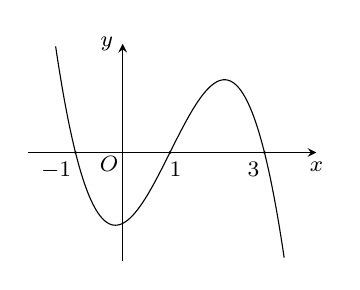
\begin{tikzpicture}[xscale=0.6, yscale=0.3, font=\footnotesize, samples=200, >=stealth]
\draw[->] (-2,0)--(4.1,0) node[below]{$x$};
\draw[->] (0,-4.6)--(0,4.6) node[left]{$y$};
\node at (0,0) [below left=-2pt]{$O$};
\draw plot[domain=-1.42:3.42] (\x,{-(\x)^3+3*(\x)^2+\x-3});
\fill[yscale=2] 
(-1,0) circle(1.0pt) node[below,xshift=-7]{$-1$}
(1,0) circle(1.0pt) node[below,xshift=2]{$1$}
(3,0) circle(1.0pt) node[below,xshift=-4]{$3$};
\end{tikzpicture}}
\loigiai{
Từ đồ thị và giả thiết, ta có bảng biến thiên của hàm số $y=f(x)$ như sau:
\begin{center}

\begin{tikzpicture}
\tkzTabInit[nocadre=true,lgt=1.2,espcl=2.5,deltacl=0.6]
{$x$/0.6,$y'$/0.6,$y$/2}
{$-\infty$,$-1$,$1$,$3$,$+\infty$}
\tkzTabLine{,+,0,-,0,+,0,-,}
\tkzTabVar{-/,+/$0$,-/,+/$0$,-/}
\end{tikzpicture}
\end{center}
Như thế $f(x) \leq 0$ với mọi $x \in \mathbb{R}$.\\
Với $y=\big[f(x)\big]^2$, ta có $y'=\left[\big(f(x)\big)^2\right]'=2f(x) \cdot f'(x)$.\\
Bảng xét dấu của $y'=\left[\big(f(x)\big)^2\right]'$:
\begin{center}

\begin{tikzpicture}
\tkzTabInit[nocadre=true,lgt=2.3,espcl=2,deltacl=0.6]
{$x$ /0.6, $f'(x)$ /0.6, $f(x)$/0.6, $\left[\big(f(x)\big)^2\right]'$ /0.9}
{$-\infty$,$-1$,$1$,$3$,$+\infty$}
\tkzTabLine{,+,0,-,0,+,0,-,}
\tkzTabLine{,-,0,-,t,-,0,-,}
\tkzTabLine{,-,0,+,0,-,0,+,}
\end{tikzpicture}
\end{center}
Như vậy hàm số $y=\big[f(x)\big]^2$ nghịch biến trên các khoảng $(-\infty;-1)$ và $(1;3)$.\\
Từ đó, số cặp số nguyên $\{a;b\}$ là số cách chọn $2$ từ $3$ số $\{1;2;3\}$ hoặc từ $10$ số $\{-10;-9;\ldots;-1\}$.\\
Số cặp số $\{a;b\}$ là $\mathrm{C}_3^2+\mathrm{C}_{10}^2=48$.
}
\end{ex}

\begin{ex}%[2-D1B5-SO-16-2425]%[VN-MT-7, Dương Phước Sang]%[2D1V5-4]
Đồ thị hàm số $y=x^3-3x^2-9x+5$ có điểm cực đại và điểm cực tiểu lần lượt là $A$ và $B$. 
Gọi $I$ là giao điểm của $AB$ với trục $Ox$. Đặt tỷ số $\dfrac{IA}{IB}=\dfrac{b}{c}$ tối giản ($b,c \in \mathbb{N}$). Tính $T=b+c$.
\par\shortans{16}
\loigiai{
Hàm số $y=x^3-3x^2-9x+5$ có tập xác định $\mathscr{D}=\mathbb{R}$.\\
$y'=3x^2-6x-9$. Cho $y'=0 \Leftrightarrow 3x^2-6x-9=0 \Leftrightarrow \hoac{&x=-1\\&x=3.}$\\
Với $x=-1$ ta có $y=y(-1)=10$. Đặt $A(-1;10)$.\\
Với $x=3$ ta có $y=y(3)=-22$. Đặt $B(3;-22)$.\\
Vì $AB$ cắt $Ox$ tại $I$ nên $\dfrac{IA}{IB}=\dfrac{\mathrm{d}(A,Ox)}{\mathrm{d}(B,Ox)}=\dfrac{\left|y_A\right|}{\left|y_B\right|}=\dfrac{10}{22}=\dfrac{5}{11}$.\\
Như vậy $b=5$ và $c=11$ nên $T=b+c=16$.
}
\end{ex}

\begin{ex}%[2-D1B5-SO-16-2425]%[VN-MT-7, Dương Phước Sang]%[2D1V3-1]
Gọi $M$, $m$ lần lượt là giá trị lớn nhất và giá trị nhỏ nhất của hàm số $y=\dfrac{3\sin x+2}{\sin x+1}$ trên đoạn $\left[ 0;\dfrac{\pi}{2} \right]$. Xác định giá trị làm tròn đến hàng phần mười của biểu thức $M^2+m^2$.
\shortans{10{,}3}
\loigiai{
Đặt $t=\sin x$, ta có $x \in \left[ 0;\dfrac{\pi}{2} \right]$ nên $t \in [0;1]$.\\
Xét hàm $f(t)=\dfrac{3t+2}{t+1}$ trên đoạn $[0;1]$ có $f'(t)=\dfrac{1}{(t+1)^2}>0,\, \forall t \in [0;1]$.\\
Suy ra hàm số $f(t)$ đồng biến trên $[0;1]$.\\
Từ đó ta có
$M=\max\limits_{[0;1]} f(t)=f(1)=\dfrac{5}{2}$
và 
$m=\min\limits_{[0;1]} f(t)=f(0)=2$.\\
Khi đó, $M^2+m^2=\left( \dfrac{5}{2} \right)^2+2^2=\dfrac{41}{4}=10{,}25 \approx 10{,}3$.
}
\end{ex}

\begin{ex}%[2-D1B5-SO-16-2425]%[VN-MT-7, Dương Phước Sang]%[2D1V3-6]
Vận tốc của một tàu con thoi từ lúc cất cánh tại thời điểm $t=0$\,s cho đến thời điểm $t=126$\,s được cho bởi công thức $v(t)=0{,}001302t^3-0{,}09029t^2+83$ (vận tốc được tính bằng đơn vị ft/s). Gọi $v_{\min}$ là vận tốc nhỏ nhất của tàu con thoi. Xác định kết quả làm tròn đến hàng phần mười của $v_{\min}$.
\shortans{18{,}7}
\loigiai{
Hàm số $v(t)=0{,}001302t^3-0{,}09029t^2+83$ liên tục trên đoạn $[0;126]$.\\
Ta có $v'(t)=0{,}003906t^2-0{,}18058t$.\\
Cho $v'(t)=0 \Leftrightarrow 0{,}003906t^2-0{,}18058t=0 \Leftrightarrow \hoac{&t=0\\&t=\dfrac{0{,}18058}{0{,}003906}.}$\\
Trên đoạn $[0;126]$, ta có 
$v(0)=83$; $v\left(\dfrac{0{,}18058}{0{,}003906}\right) \approx 18{,}67301185$; $v(126) \approx 1254{,}045512$.\\
Tàu con thoi đạt vận tốc nhỏ nhất bằng $v\left(\dfrac{0{,}18058}{0{,}003906}\right) \approx 18{,}7$ ft/s.
}
\end{ex}

\begin{ex}%[2-D1B5-SO-16-2425]%[VN-MT-7, Dương Phước Sang]%[2D1H4-1]
Một mảnh vườn hình chữ nhật có diện tích bằng $900$\,m$^2$. Biết chiều dài của mảnh vườn là $x$\,(m). Gọi biểu thức tính chu vi của mảnh vườn là $P(x)$\,(m). Biết rằng phương trình tiệm cận xiên của đồ thị hàm số $P(x)$ là $y=ax+b$. Tính giá trị biểu thức $T=10^a+b$.
\shortans{100}
\loigiai{
Mảnh vườn có chiều dài $x$\,(m) nên có chiều rộng là $\dfrac{900}{x}$\,(m).\\
Điều kiện: $x \geq \dfrac{900}{x} \Leftrightarrow x \geq 30$.\\
Ta có $P(x)=2\left( x+\dfrac{900}{x} \right)=2x+\dfrac{1800}{x}$.\\
Vì $\lim\limits_{x \to +\infty} [P(x)-2x]=\lim\limits_{x \to +\infty} \dfrac{1800}{x}=0$ nên đồ thị hàm số $P(x)$ có tiệm cận xiên là đường thẳng $y=2x$.\\
Suy ra $a=2$, $b=0$. Do vậy, $T=100$.
}
\end{ex}

\begin{ex}%[2-D1B5-SO-16-2425]%[VN-MT-7, Dương Phước Sang]%[2D1V5-4]
Biết rằng đồ thị hàm số $y=\dfrac{x+1}{x-1}$ cắt đường thẳng $y=2x-1$ tại hai điểm phân biệt $A$, $B$. Tính diện tích tam giác $OAB$.
\shortans{1}
\loigiai{
Phương trình hoành độ giao điểm của đồ thị hai hàm số $y=\dfrac{x+1}{x-1}$ và $y=2x-1$ là
\[\dfrac{x+1}{x-1}=2x-1 \Leftrightarrow 2x^2-4x=0 \Leftrightarrow \hoac{&x=0\\&x=2.}\]
Suy ra toạ độ các giao điểm của đồ thị hai hàm số đó là $A(0;-1)$, $B(2;3)$.\\
Diện tích cần tìm là 
$S=\dfrac{1}{2}|0 \cdot 3-(-1) \cdot 2|=1$.
}
\end{ex}
\Closesolutionfile{ans}
\begin{indapan}
	{ans/ans\currfilebase}
\end{indapan}

